\begin{figure}[!htb]
\begin{center}
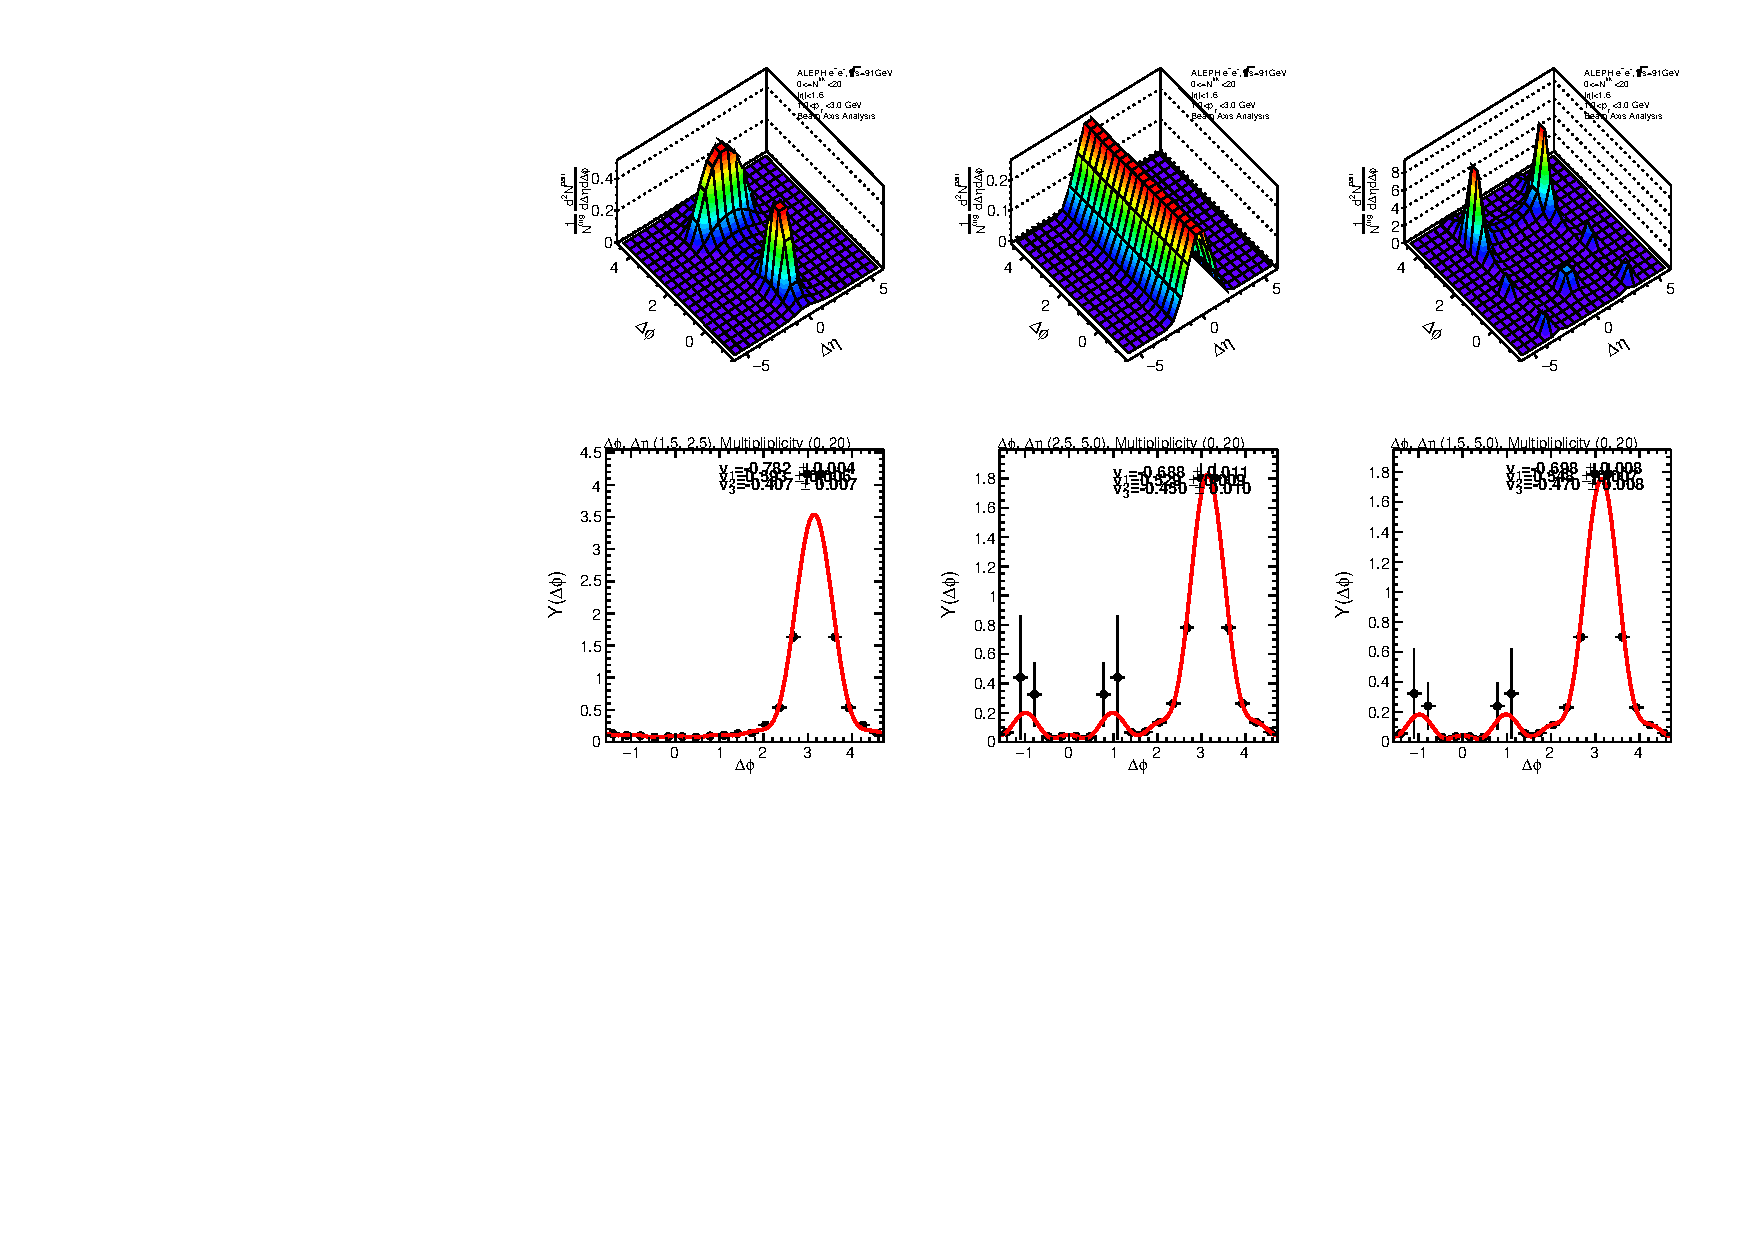
\includegraphics[width=.45\textwidth]{images/BeamAxis/0_20_2/beam/LEP1Data1992_thrust0_mix0_wta0_perp0_gen0_ajrej0_ajrejcut0p0_threejet0_threejetcut0p0_owbarrel0_anatyperegion0_etabarrelcut0p0_typeEnergyBarrelSel0_etabarrelcutforEselection0p0_maxrelenergyinsidebarrel1p0_typemultiplicity0_ASummary_0_0_20_2_0.pdf}
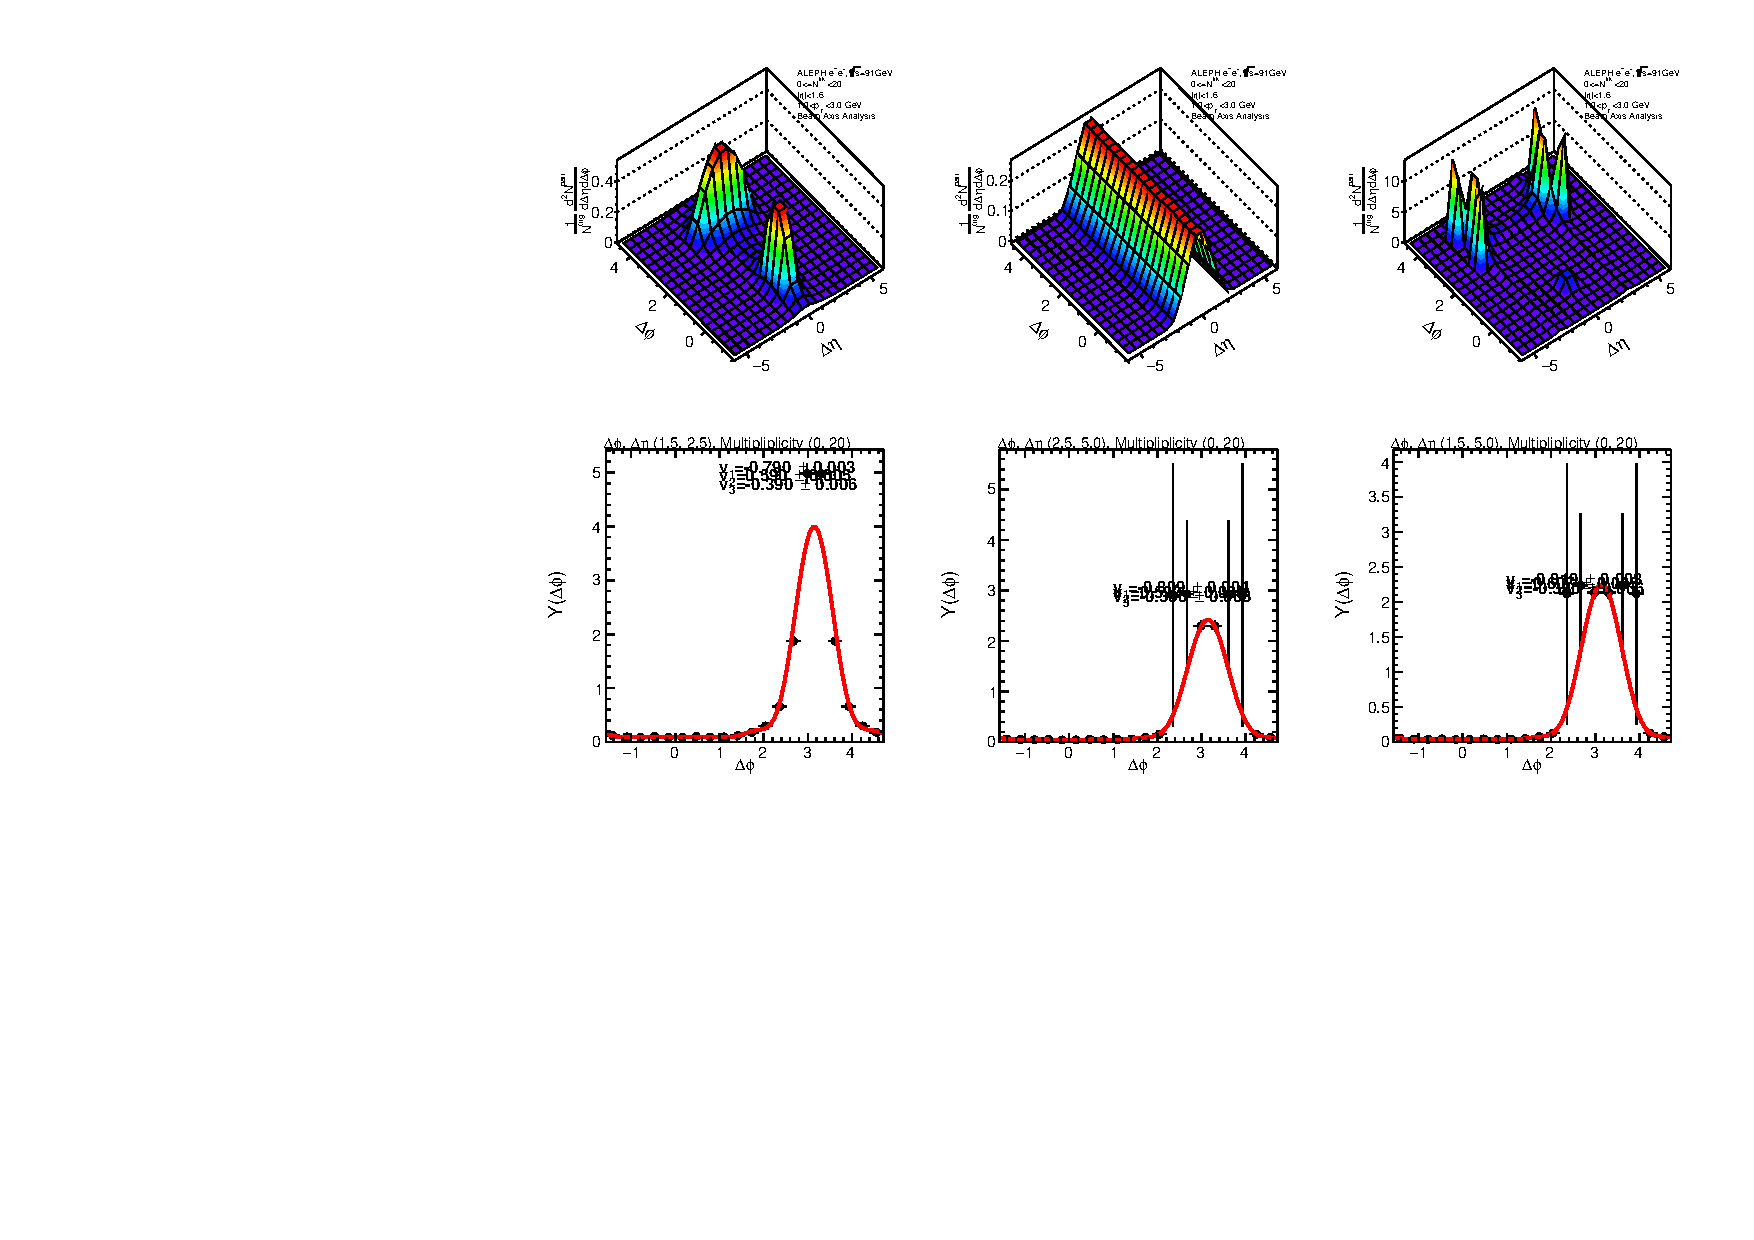
\includegraphics[width=.45\textwidth]{images/BeamAxis/0_20_2/beam/LEP1MC1994_20180323_thrust0_mix0_wta0_perp0_gen0_ajrej0_ajrejcut0p0_threejet0_threejetcut0p0_owbarrel0_anatyperegion0_etabarrelcut0p0_typeEnergyBarrelSel0_etabarrelcutforEselection0p0_maxrelenergyinsidebarrel1p0_typemultiplicity0_ASummary_0_0_20_2_0.pdf}
\caption{Two-particle correlation functions as a function of  $\Delta\phi$ in $e^{+}e^{-}$ with particle multiplicity $<$ 20 for data and MC respectively.}
\label{fig:ProjectionMultLess20} 
\end{center}
\end{figure}


\begin{figure}[!htb]
\begin{center}
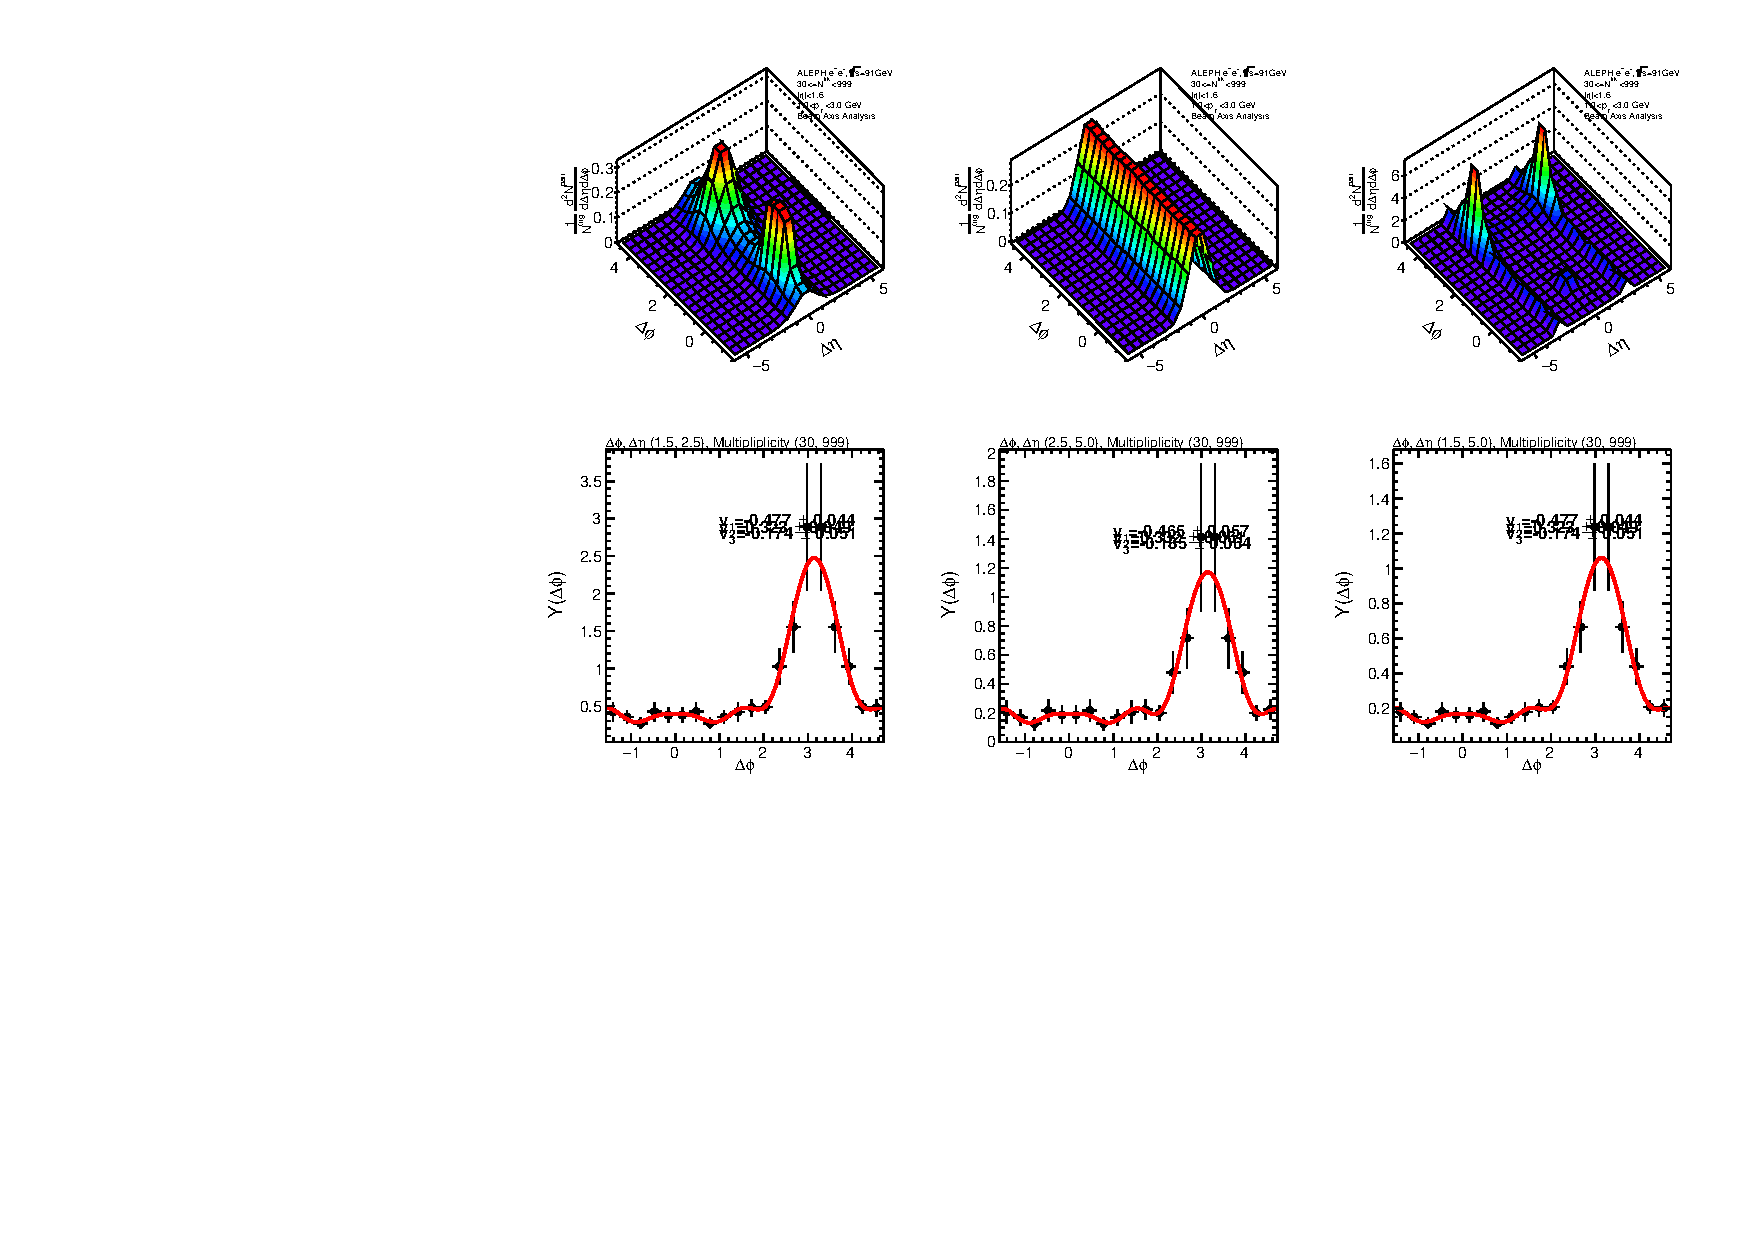
\includegraphics[width=.45\textwidth]{images/BeamAxis/30_999_2/beam/LEP1Data1992_thrust0_mix0_wta0_perp0_gen0_ajrej0_ajrejcut0p0_threejet0_threejetcut0p0_owbarrel0_anatyperegion0_etabarrelcut0p0_typeEnergyBarrelSel0_etabarrelcutforEselection0p0_maxrelenergyinsidebarrel1p0_typemultiplicity0_ASummary_0_30_999_2_0.pdf}
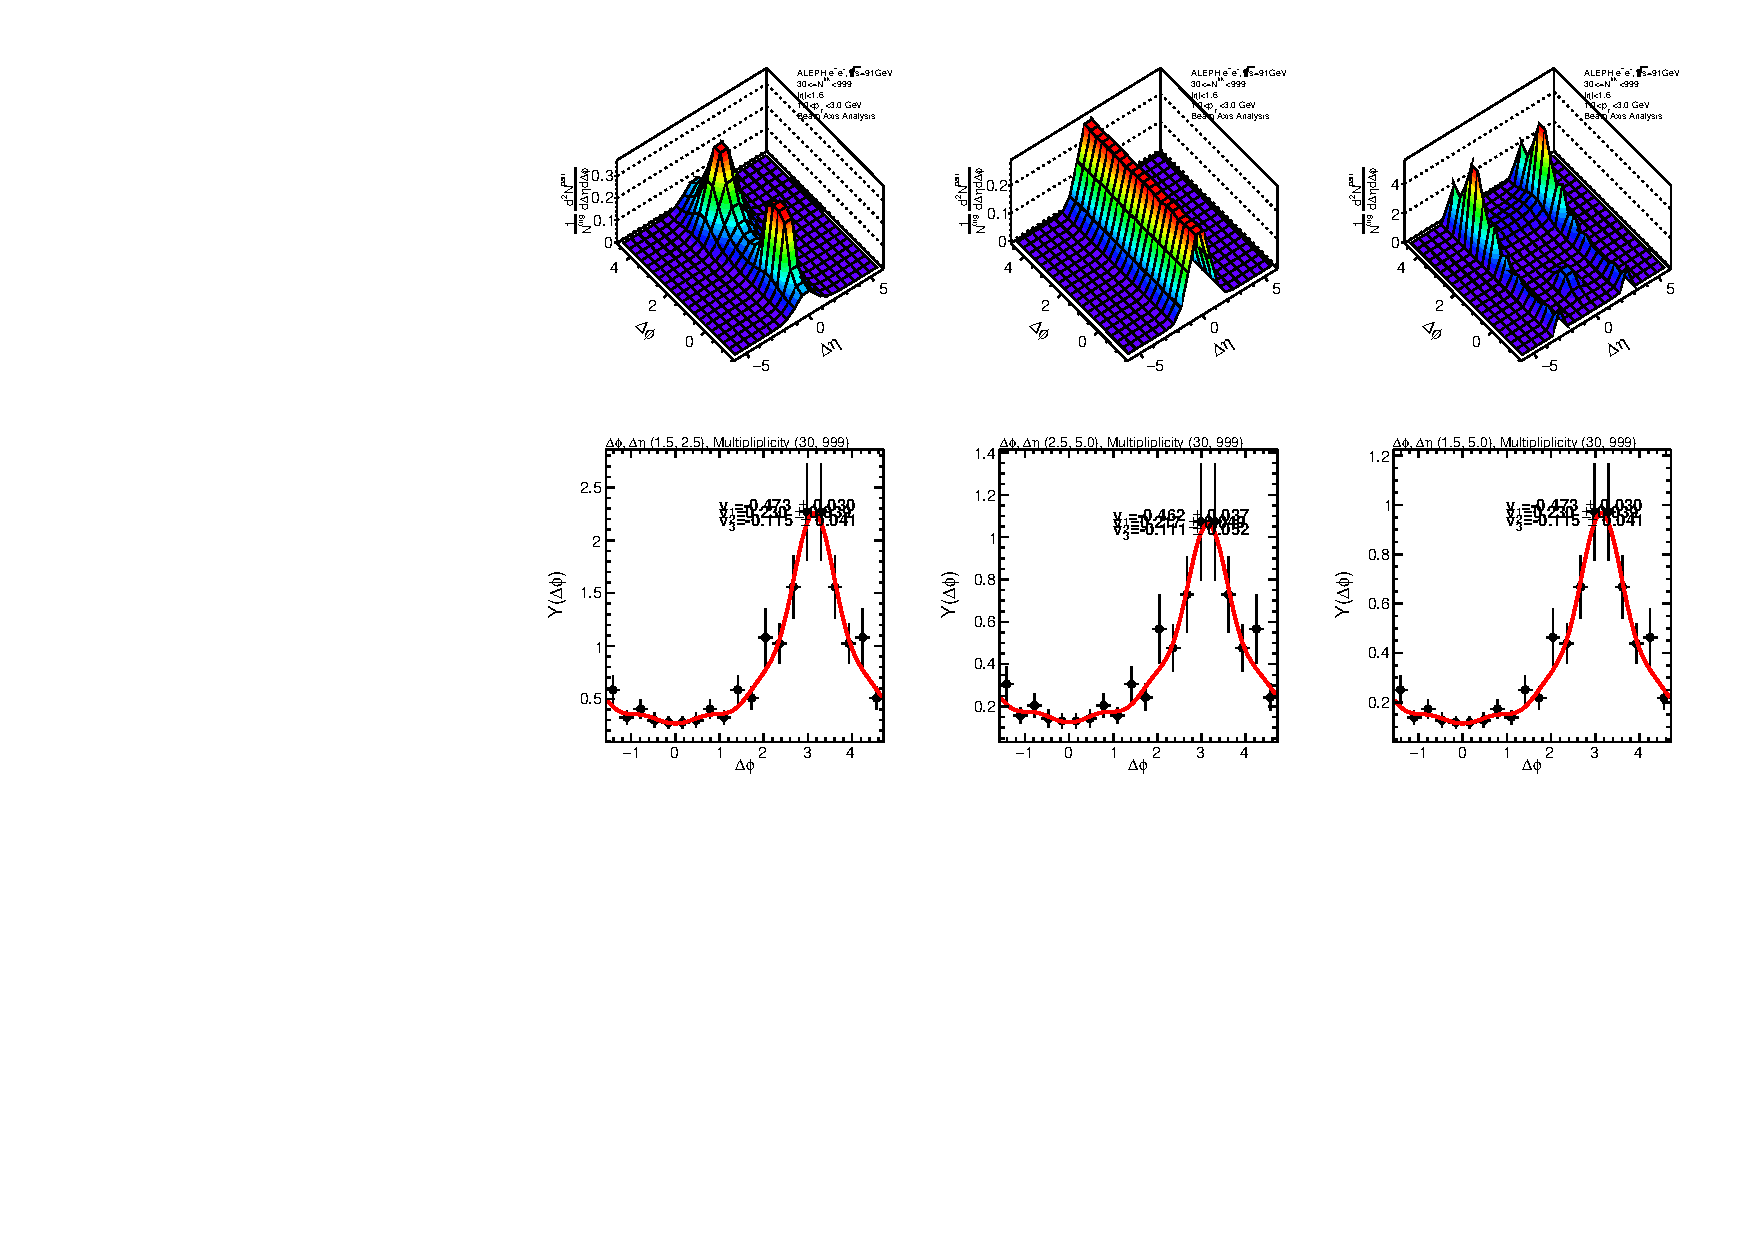
\includegraphics[width=.45\textwidth]{images/BeamAxis/30_999_2/beam/LEP1MC1994_20180323_thrust0_mix0_wta0_perp0_gen0_ajrej0_ajrejcut0p0_threejet0_threejetcut0p0_owbarrel0_anatyperegion0_etabarrelcut0p0_typeEnergyBarrelSel0_etabarrelcutforEselection0p0_maxrelenergyinsidebarrel1p0_typemultiplicity0_ASummary_0_30_999_2_0.pdf}
\caption{Two-particle correlation functions as a function of  $\Delta\phi$ in $e^{+}e^{-}$ with particle multiplicity $>$ 30 for data and MC respectively.}
\label{fig:ProjectionMultBigger30} 
\end{center}
\end{figure}
